\chapter{Image import}

InVesalius imports files in DICOM format, including compressed files (lossless JPEG), Analyze (Mayo Clinic) $^\copyright$, NIfTI, PAR/REC, BMP, TIFF, JPEG and PNG formats.

\section{DICOM}

On menu \textbf{File}, click on \textbf{Import DICOM...}. If you prefer, use the shortcut of keyboard \textbf{Ctrl + I}. Import DICOM images can also be triggered by the toolbar icon described in the figure~\ref{fig:import}.

\begin{figure}[!htb]
\centering

\includegraphics[scale=0.2]{file_import_original.png}
\caption{Shortcut to DICOM import}
\label{fig:import}
\end{figure}

\hspace{.2cm}

Then select the directory containing the DICOM files, as in figure~\ref{fig:win_folder}. InVesalius will search for files also in subdirectories of the chosen directory, if they exist.

\newpage

Click on \textbf{OK} button.

\begin{figure}[!htb]
\centering
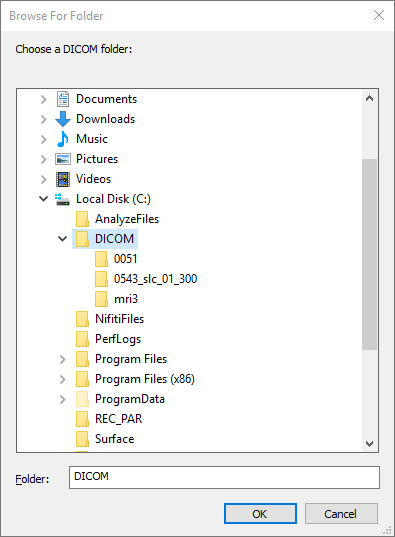
\includegraphics[scale=0.5]{import_select_folder_en.png}
\caption{Folder Selection}
\label{fig:win_folder}
\end{figure}

\hspace{.2cm}

While InVesalius search for DICOM files in the directory, the loading progress of the scanned files is displayed, as shown in the figure~\ref{fig:ver_file}.

\begin{figure}[!htb]
\centering
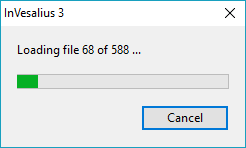
\includegraphics[scale=0.6]{import_load_files_en.png}
\caption{Loading file status}
\label{fig:ver_file}
\end{figure}

\newpage

If DICOM files are found, a window open (figure~\ref{fig:win_import}) to select the patient and the respective series to be opened. It is also possible to skip images for reconstruction.

\begin{figure}[!htb]
\centering
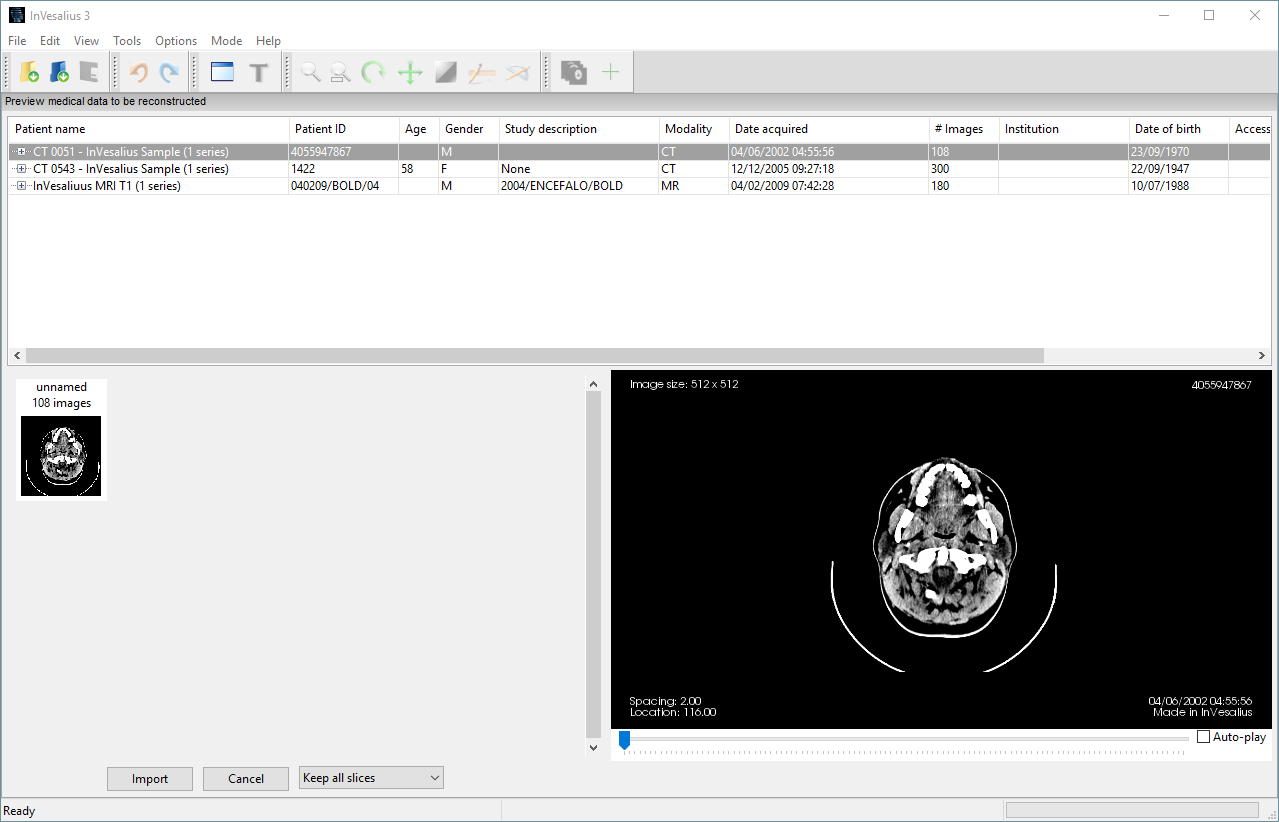
\includegraphics[scale=0.4]{import_window_en.png}
\caption{Import window}
\label{fig:win_import}
\end{figure}

\newpage

If you want to import a series with all the images present, click "\textbf{+}" on the side patient's name to expand the series belonging to him. \textbf {Double-click} with left mouse button on the description of the series. See figure~\ref{fig:import_serie}.

\begin{figure}[!htb]
\centering
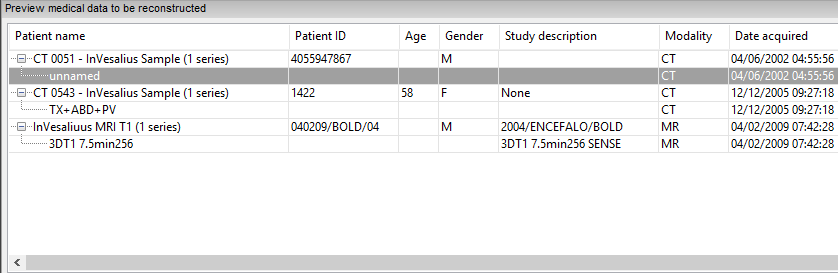
\includegraphics[scale=0.5]{import_window_detail_en.png}
\caption{Series selection}
\label{fig:import_serie}
\end{figure}
 
Some cases in particular when there is no computer with memory and/or satisfactory processing to work with many images in a series, can be it is recommended to skip (skip) some of them. To do this, click \textbf {once} with the \textbf{left} of the mouse over the description of the series (figure~\ref{fig:import_serie}) and select how many images will be skipped (figure~\ref{fig:skip_image}). Click on~\textbf {Import} button.

\begin{figure}[!htb]
\centering
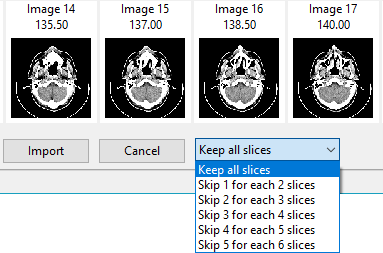
\includegraphics[scale=0.6]{import_window_skip_slice_en.png}
\caption{Skip imagens option}
\label{fig:skip_image}
\end{figure}

If insufficient amount of available memory is detected at the time of loading the images it is recommended reduce the resolution of the slices to work with volumetric and surface visualization, as shown in the \ref{fig:resize_image} window.
The slices will be resized according to the percentage relative to the original resolution. For example, if each slice of the exam contains the dimension of 512 x 512 pixels and the "Percentage of original resolution" is suggested to be 60 \%, each resulting image will be 307 x 307 pixels. If you want to open with the original resolution select the value 100.

\begin{figure}[!htb]
\centering
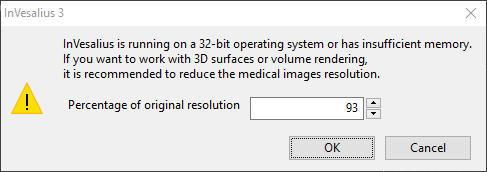
\includegraphics[scale=0.5]{import_window_lower_memory_en.png}
\caption{Image size reduction}
\label{fig:resize_image}
\end{figure}

After the previous procedures, a window will be displayed (figure \ref{fig:prog_recons}) with progress reconstruction (when images are stacked and interpolated).

\begin{figure}[!htb]
\centering
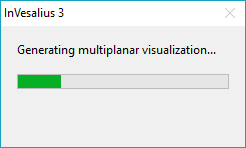
\includegraphics[scale=0.6]{import_window_progress_en.png} 
\caption{Reconstruction progress}
\label{fig:prog_recons}
\end{figure}

\newpage

\section{Analyze}

To import Analyze files, on menu \textbf{File}, click on \textbf{Importar other files...}, then click in the \textbf{Analyze} option as show the figure~\ref{fig:analyze_menu}.

\begin{figure}[!htb]
\centering
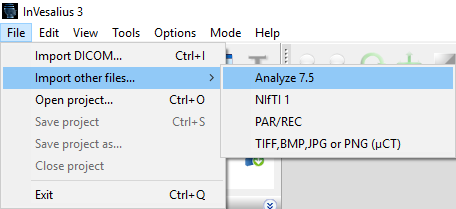
\includegraphics[scale=0.4]{import_analyze_menu_en.png}
\caption{Menu for importing images in analyze format.}
\label{fig:analyze_menu}
\end{figure}

Select the file of Analyze format, in extension \textbf{.hdr} and click on \textbf{Open} button (Figure \ref{fig:analyze_import}).
 
\begin{figure}[!htb]
\centering
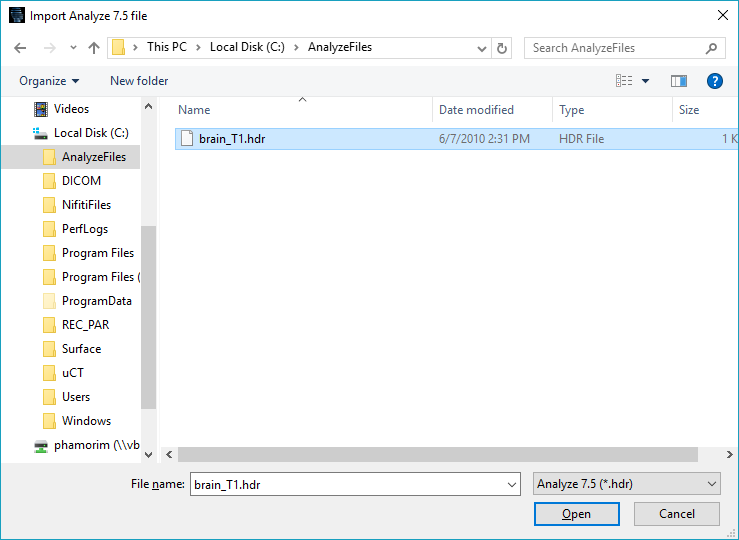
\includegraphics[scale=0.4]{import_analyze_window_en.png}
\caption{Import analyze file format}
\label{fig:analyze_import}
\end{figure}

\section{NIfTI}

To import NIfTI files, on menu \textbf{File}, click on option \textbf{Import other files...} and then click on \textbf{NIfTI} option as shown figure~\ref{fig:import_nifti_menu_pt}.


\begin{figure}[!htb]
\centering
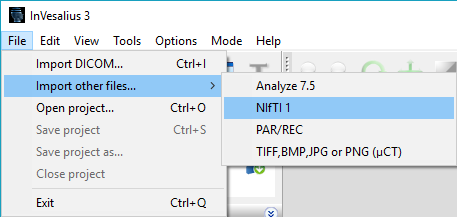
\includegraphics[scale=0.4]{import_nifti_menu_en.png}
\caption{Menu to import images in NIfTI format}
\label{fig:import_nifti_menu_pt}
\end{figure}

Select the file of type NIfTI, on \textbf{nii.gz} or \textbf{.nii} extension, click on \textbf{Open} (figure \ref{fig:import_nifti_window_pt}). If the file is in another extension as \textbf{.hdr}, select \textbf{all files(*.*)} option.

\begin{figure}[!htb]
\centering
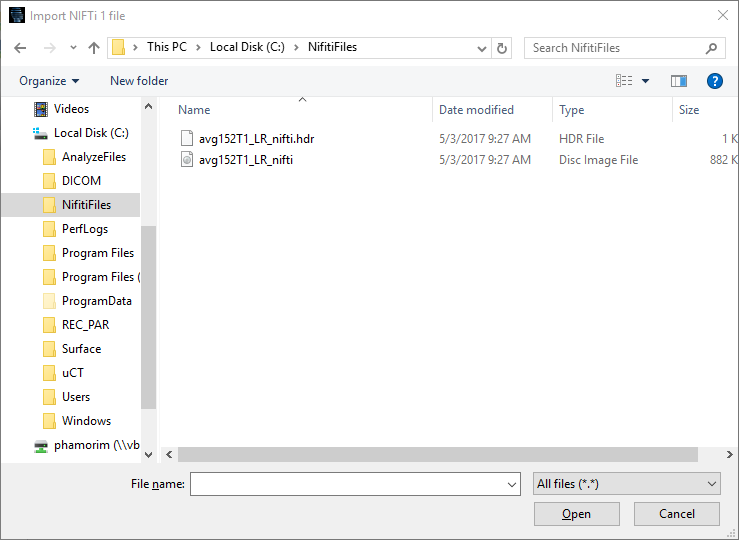
\includegraphics[scale=0.4]{import_nifti_window_en.png}
\caption{Importing images in NIfTI format.}
\label{fig:import_nifti_window_pt}
\end{figure}

\section{PAR/REC}

To import PAR/REC file, on main menu, click on \textbf{File}, \textbf{Import other files...} option and then click on \textbf{PAR/REC} as shown the figure \ref{fig:import_parrec_menu_pt}.

\begin{figure}[!htb]
\centering
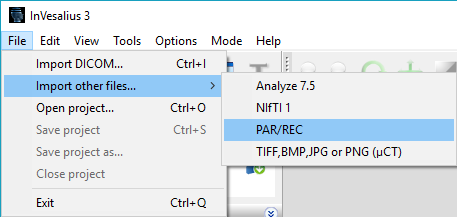
\includegraphics[scale=0.4]{import_parrec_menu_en.png}
\caption{Menu for importing PAR/REC images}
\label{fig:import_parrec_menu_pt}
\end{figure}

Select PAR/REC file type, in extension \textbf{.par} and click on \textbf{Open} (figure~\ref{fig:import_parrec_window_pt}). If the file has no extension, select \textbf{all files(*.*)} option.

\begin{figure}[!htb]
\centering
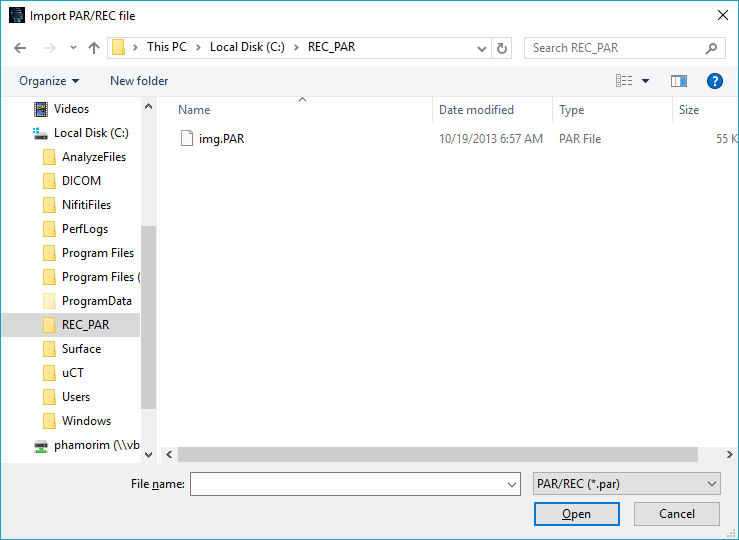
\includegraphics[scale=0.4]{import_parrec_window_en.png}
\caption{PAR/REC import}
\label{fig:import_parrec_window_pt}
\end{figure}

\section{TIFF, JPG, BMP, JPEG or PNG (micro-CT)}

TIFF, JPG, BMP, JPEG or PNG file format for reconstruction can be provided with microtomography equipment (micro-CT or $\mu$CT) or others. InVesalius imports files in these formats if pixels present are represented in \textbf{grayscale}.

To import, click on menu \textbf{File}, \textbf{Import other files...} and then click on \textbf{TIFF, JPG, BMP, JPEG ou PNG ($\mu$CT)} option as shown the figure~\ref{fig:import_bmp_menu_pt}.

\begin{figure}[!htb]
\centering
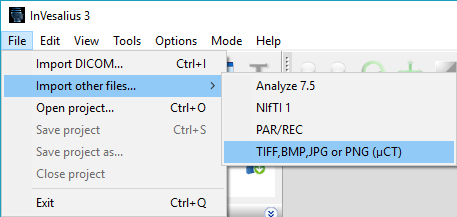
\includegraphics[scale=0.4]{import_bmp_menu_en.png}
\caption{Import images in BMP and others formats}
\label{fig:import_bmp_menu_pt}
\end{figure}

Select the directory that contains the files, as shown the figure~\ref{fig:import_bmp_select_folder}. InVesalius will search for files also in subdirectories of the chosen directory, if they exist. 

Click on \textbf{OK} button.

\begin{figure}[!htb]
\centering
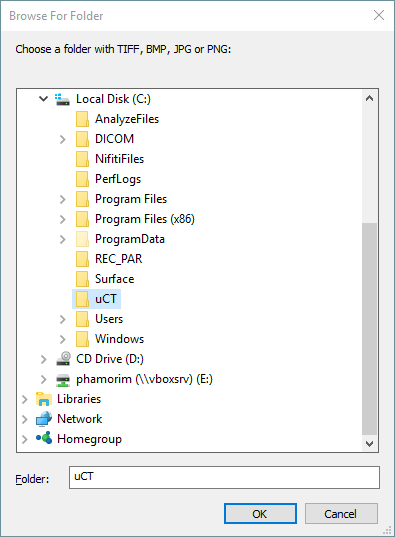
\includegraphics[scale=0.5]{import_bmp_select_folder_en.png}
\caption{Folder selection}
\label{fig:import_bmp_select_folder}
\end{figure}

While InVesalius looking for TIFF, JPG, BMP, JPEG, or PNG files in the directory, the upload progress of the scanned files is displayed, as illustrated by the \ref{fig:import_bmp_load_pt} figure.

\begin{figure}[!htb]
\centering
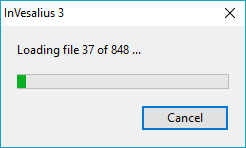
\includegraphics[scale=0.6]{import_bmp_load_en.png}
\caption{Checking and loading files status.}
\label{fig:import_bmp_load_pt}
\end{figure}

If files of type TIFF, JPG, BMP, JPEG or PNG are founded, a window open (figure~\ref{fig:import_bmp_window_pt}) to display the founded files eligible for reconstruction. You can also skip images to rebuild or remove files from the rebuild list. The files are sorted according to the file name, it is recommended to use numbers in their names according to the order you want to get in the rebuild.

\begin{figure}[!htb]
\centering
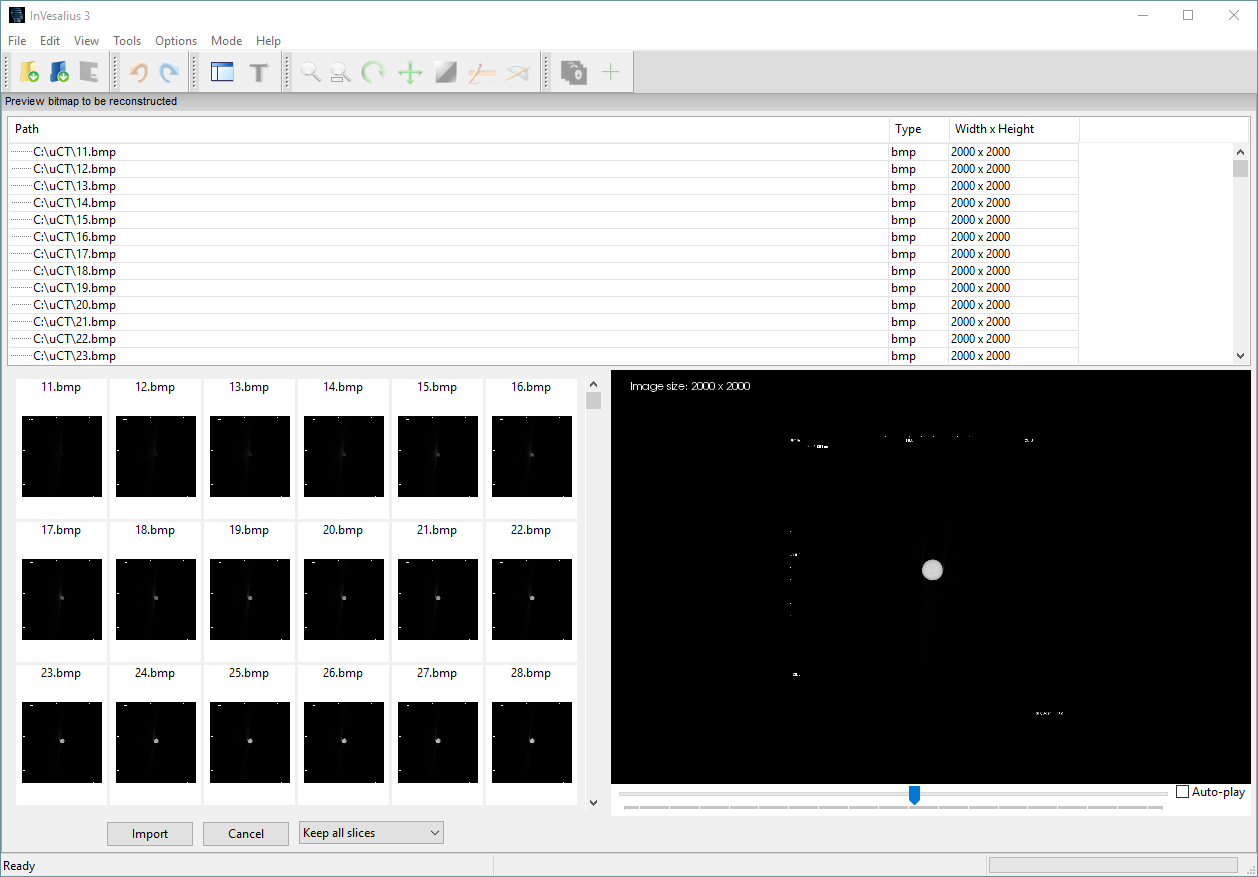
\includegraphics[scale=0.3]{import_bmp_window_en.png}
\caption{Window to import BMP files.}
\label{fig:import_bmp_window_pt}
\end{figure}
 
To delete files that are not of interest, you can select a file by clicking the \textbf{left mouse button} and then pressing the \textbf{delete} key. You can also choose a range of files to delete, so you need to click the \textbf{left mouse button} on the first file in the track, hold down the \textbf{shift} key, click again with the \textbf{button Left mouse button} in the last file of the track and finally press the \textbf{delete} button.
 
Like importing DICOM files module, you can skip BMP images for rebuilding. In some cases, particularly where a computer with satisfactory memory and/or processing is not available to work with many images in a series, it may be advisable to skip (skip) some of them. To do this, select how many images to skip (figure~\ref{fig:import_bmp_skip_pt}). Click \textbf{Import} button.

\begin{figure}[!htb]
\centering
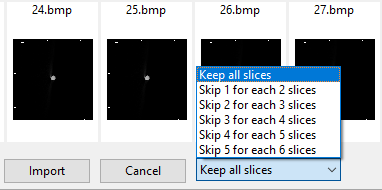
\includegraphics[scale=0.4]{import_bmp_skip_en.png}
\caption{Importation window}
\label{fig:import_bmp_skip_pt}
\end{figure}

To reconstruct this file type, it is necessary to define a name for the project, to indicate the orientation of the images (axial, coronal or sagittal), voxel spacing ($X$, $Y$ and $Z$) in \textbf{mm} as shown in the figure~\ref{fig:import_bmp_spacing_pt}. The voxel spacing in $X$ is the pixel width of each image, $Y$ the pixel length, and $Z$ represents the distance of each slice (voxel height).

If the image set consists of microtomography images, more specifically GE and Brucker equipment, it is possible that InVesalius will read the text file with the acquisition parameters that normally stay in the same folder as the images and automatically insert the spacing . This verification can be done when the values of $X$, $Y$ and $Z$ are different from "1.00000000", otherwise it is necessary to enter the values of the respective spacing.

\textbf{Attention, the spacing is a paramount parameter for the correct dimension of the objects in the software. Incorrect spacing will provide incorrect measurements.}

Once you have completed all the parameters, just click the \textbf{Ok} button.

\begin{figure}[!htb]
\centering
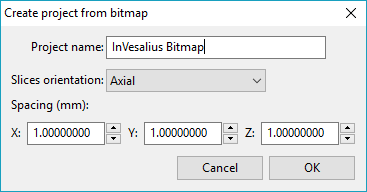
\includegraphics[scale=0.5]{import_bmp_spacing_en.png}
\caption{Tela de importação}
\label{fig:import_bmp_spacing_pt}
\end{figure}

If insufficient memory is available when loading images, it is recommended to reduce the resolution of the slices to work with volumetric and surface visualization, as shown in the \ref{fig:import_bmp_resize_pt} window. The slices will be resized according to the percentage relative to the original resolution. For example, if each slice of the exam contains the dimension of 512 x 512 pixels and the "Percentage of the original resolution" is suggested at 60\%, each resulting image will have 307 x 307 pixels. If you want to open with the original resolution select the value 100.

\begin{figure}[!htb]
\centering
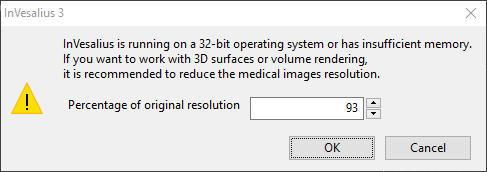
\includegraphics[scale=0.5]{import_window_lower_memory_en.png}
\caption{Image resize}
\label{fig:import_bmp_resize_pt}
\end{figure}

If the image was obtained with the gantry tilted it will be necessary to do a correction to avoid deformations on the reconstruction. InVesalius allows the user do this correction. When importing an image with the gantry tilted it will be shown a dialog with the degree of tilt (figure~\ref{fig:gantry_tilt}). It is possible to change this value, but it is not recommended. Click on the \textbf{Ok} button to do the correction. If you click on the \textbf{cancel} button the correction will not be done.

\begin{figure}[!htb]
\centering
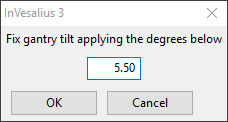
\includegraphics[scale=0.75]{window_gantry_tilt_en.png}
\caption{Redimensionamento de imagens}
\label{fig:gantry_tilt}
\end{figure}

%Após os passos anteriores é necessário aguardar um instante para completar a reconstrução multiplanar conforme mostra a figura~\ref{fig:import_bmp_mpr_pt.png}.

After the previous steps it is necessary to wait a moment to complete the multiplanar reconstruction as shown in the figure~\ref{fig:import_bmp_mpr_pt.png}.

\begin{figure}[!htb]
\centering
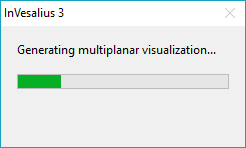
\includegraphics[scale=0.6]{import_window_progress_en.png}
\caption{Multiplanar reconstruction in progress.}
\label{fig:import_bmp_mpr_pt.png}
\end{figure}
